\documentclass[10pt,twocolumn]{article}
\usepackage[margin=0.75in,columnsep=0.3in]{geometry}
\usepackage{booktabs}
\usepackage{graphicx}
\usepackage{amsmath}
\usepackage{xcolor}
\usepackage[font=small,labelfont=bf]{caption}
\usepackage[colorlinks=true,linkcolor=black,citecolor=blue!50!black,urlcolor=blue!50!black]{hyperref}
\usepackage{etoolbox}
\makeatletter
\AtBeginEnvironment{itemize}{\setlength{\itemsep}{0pt}\setlength{\parsep}{0pt}\setlength{\topsep}{2pt}\setlength{\leftmargin}{1.4em}}
\AtBeginEnvironment{description}{\setlength{\itemsep}{0pt}\setlength{\parsep}{0pt}\setlength{\topsep}{2pt}}
\makeatother
\setlength{\parskip}{0pt}
\setlength{\parindent}{1em}

\title{Checking the Answer, Not the Model: Data-Level Signals\\ for Trustworthy Text-to-SQL Analytics\\[2pt]\large (Work in Progress)}
\author{Anonymous Authors\\ \small StateSync project (author names to be added)}
\date{Draft, 30 September 2026}

\begin{document}
\maketitle

\begin{abstract}
Text-to-SQL systems sometimes return answers that are wrong but plausible, and a user reading the prose cannot tell which. Recent work predicts correctness from the model: sampling agreement, log-probabilities or a second model acting as judge. We describe StateSync, a self-hosted analytics assistant that instead checks the answer against the data, without a model call. It assigns each answer an evidence tier, runs deterministic checks (a join fan-out probe, truncation and NULL warnings) and traces every number in the prose to its source. We report two preliminary results. On a 30-question baseline the system answers 25 correctly. In a pilot over stored answers, figure grounding traced 97.5\% of 1,939 figures and flagged 8 of 944 analysable answers; the pilot is in-sample, because checker defects were found and fixed on the same data. Nothing has yet been measured on an external benchmark. We describe a pre-registered plan using BIRD Mini-Dev with corrected annotations, and state its hypotheses before any measurement.
\end{abstract}

\section{Introduction}
A text-to-SQL assistant fails in a particular way. When the query is wrong, the answer is usually still well formed: a number, a sentence and a table. A join that repeats rows inflates a sum; a follow-up question counts at the wrong grain; a sentence restates a figure the result does not contain. In a 2026 report by dbt Labs, 71\% of respondents named incorrect or hallucinated outputs reaching stakeholders as a top concern \cite{dbt2026report}.

One line of work asks how to predict, from the model's behaviour, whether an answer is correct. Richardson \cite{richardson2026} studies this as selective prediction. Black-box signals reach 0.61--0.68 AUROC, log-probability 0.67, single LLM judges 0.72 (GPT-4o-mini) and 0.78 (Claude), and a two-provider judge ensemble 0.82. Fine-tuned verifiers drop to about 0.66 on unseen schemas. These signals cost extra model calls and are themselves fallible.

We take a complementary route: check the answer against the data. Many errors leave evidence in the executed result: a count that differs from a distinct count, a result cut at the row limit, a figure in the prose that appears nowhere in the result. Such checks need no model, add no token cost, and can be stated as exact rules. Their weakness is coverage: they cannot see that a filter value was wrong if the result is internally consistent.

This paper is a work-in-progress report. Its contributions are:
\begin{itemize}
\item a system that labels each answer with an \emph{evidence tier} and runs \emph{deterministic checks} on the executed result (Section~\ref{sec:system});
\item \emph{figure grounding}, a model-free procedure that traces each number in an answer to its source and turns untraced numbers into a caveat;
\item a \emph{pilot} of figure grounding over 944 stored answers, with a manual review of every flag, and a 30-question baseline (Section~\ref{sec:results});
\item a \emph{pre-registered evaluation plan} on BIRD Mini-Dev with corrected annotations, with research questions and hypotheses fixed before measurement (Section~\ref{sec:plan}).
\end{itemize}
We state plainly what is not yet measured in Section~\ref{sec:limits}.

\section{System}\label{sec:system}
StateSync answers natural-language questions over a Postgres database and uploaded documents.

\paragraph{Pipeline and security split.} A question is normalised, follow-ups are rewritten into standalone questions, and a router chooses SQL, documents or a hybrid path. A SQL agent drafts a query, with a correction loop of up to 3 retries and a SQL gate. A synthesizer writes the prose, with citations built in code, and deterministic checks run last. The orchestrator, which is the model-facing side, holds no database credentials. A separate MCP service is the only credential holder, and it passes every query through a three-layer gate: a parse (pglast) that requires exactly one SELECT, no data-modifying CTEs and no denied functions; a READ ONLY transaction that is always rolled back; and a read-only database role. Row-level security applies to every application table.

\paragraph{Evidence tiers.} The tier of an answer is a pure function of what ran (Table~\ref{tab:tiers}). \emph{Compiled} answers reuse an owner-approved query: literals in the approved SQL become typed slots via the Postgres parser, and values are filled in by code, so no SQL-model call is made.

\begin{table}[t]
\centering\small
\caption{Evidence tiers, from strongest to weakest.}\label{tab:tiers}
\begin{tabular}{@{}lp{5.4cm}@{}}
\toprule
Tier & What ran \\
\midrule
verified & owner-approved SQL, run as is \\
compiled & template derived from approved SQL; values filled in code; no SQL-model call \\
checked & new SQL; deterministic checks on; no caveat raised \\
unchecked & none of the above \\
\bottomrule
\end{tabular}
\end{table}

\paragraph{Deterministic checks.} Three checks run on the executed result and the prose.
\begin{itemize}
\item \emph{Fan-out probe.} For SUM or AVG over a join, the probe compares \texttt{COUNT(key)} with \texttt{COUNT(DISTINCT key)} on the joined rows. A mismatch means rows were repeated.
\item \emph{Truncation and NULL.} Warns when the result was cut at the row limit, or when an aggregate runs over mostly-NULL values.
\item \emph{Figure grounding.} Every number in the prose is matched, within the rounding its own digits imply (``1.2M'' covers 1.15M to 1.25M), to one of these sources: a result cell (fractions written as percentages count); a column sum, average, minimum or maximum, or the row count; part of a text value; a number in the question; a number in a cited passage; or a ratio or difference of two figures already traced. Years, dates, identifiers and list markers are excluded. Unmatched figures become a caveat and move the answer out of the ``checked'' tier. The interface marks each figure with its source on hover.
\end{itemize}

\paragraph{Self-testing workspace.} Approved queries are re-run on a schedule with no model. The result shape signature (column names and whether rows return) is compared with the stored one to detect schema drift.

\paragraph{Quote-verified definitions.} Business definitions are mined from uploaded documents. Code pre-selects passages by definitional wording within a character budget. The model must quote the exact sentence, and a proposal is kept only if the normalised quote occurs in the cited passage and contains the term. In two live runs, on a handbook with four definitions and on a demo handbook with seven, the system returned 4 of 4 and 7 of 7 definitions, none invented and none dropped, each in 1 model call. These are spot checks, not an evaluation. Connecting an owner's own database is likewise gated: the login is saved only if it is provably read-only, and a live check of this gate passed 24 of 24 cases.

\section{Preliminary Results}\label{sec:results}
All results in this section are preliminary. Neither has been run on an external benchmark.

\subsection{Baseline: 30 questions}
The baseline uses Groq gpt-oss-120b for SQL. It comprises 30 questions: 10 over real e-commerce data (olist), 8 SQL questions over a synthetic logistics corpus, 6 over documents and 6 follow-ups. The system answered 25 of 30 correctly (83\%), and routed all 30 correctly (Table~\ref{tab:baseline}). A question costs on average 4.7 model calls and about 5,000 tokens (4,652 in, 356 out). Latency is 2.6\,s at the median and 3.5\,s at the 90th percentile. The baseline ran at the shipped settings of the time, with the deterministic answer checks switched off, so it measures answer correctness only, not the checks.

\begin{table}[t]
\centering\small
\caption{Baseline correctness by category (30 questions, one run).}\label{tab:baseline}
\begin{tabular}{@{}lrr@{}}
\toprule
Category & Questions & Correct \\
\midrule
olist (real data) & 10 & 10 \\
Logistics SQL (synthetic) & 8 & 6 \\
Documents & 6 & 5 \\
Follow-ups & 6 & 4 \\
\midrule
All & 30 & 25 (83\%) \\
\bottomrule
\end{tabular}
\end{table}

The five misses were: an ambiguous denominator (``what percentage of fulfillments were delivered late'': the generated SQL divides by all fulfillments, the reference by delivered ones); a projection difference; one document retrieval miss; and two follow-ups that counted at the wrong grain. In the first of these two, payment rows were counted instead of orders. In the second, a join duplicated reviews under \texttt{COUNT(*)}. The fan-out probe covers only SUM and AVG so far, so it would not have flagged the second.

\subsection{Pilot: figure grounding over stored answers}
We ran figure grounding, with zero model calls, over every stored conversation turn that has executed SQL and an answer: 1,268 turns. Of these, 944 were analysable; 319 had no result columns and 5 had result previews truncated below the row count.

\begin{table}[t]
\centering\small
\caption{Figure-grounding pilot. \emph{After fixes} follows repairs of two checker defects and the addition of derived ratios and differences. In-sample.}\label{tab:pilot}
\begin{tabular}{@{}lrr@{}}
\toprule
 & First run & After fixes \\
\midrule
Figures & 2,024 & 1,939 \\
Traced & 91.8\% & 97.5\% \\
Answers flagged & 29 (3.1\%) & 8 (0.85\%) \\
\bottomrule
\end{tabular}
\end{table}

\paragraph{Manual review of flags.} We reviewed all 29 first-run flags by hand. Twenty-one were false alarms from two defects of the checker: numbers inside text values (for example ``Seller Store 28'' and ``port=5432'') and dates written with Unicode non-breaking hyphens. After fixing both, and counting ratios and differences of traced figures as derived (a source that matched no figure in this pilot), 8 answers were flagged (Table~\ref{tab:pilot}). All 8 are genuinely not supported by their own result: 6 are follow-ups that repeat figures from an earlier turn, 1 is a hybrid answer quoting document figures (the pilot did not pass the passages to the checker), and 1 described a method instead of answering. Figure~\ref{fig:sources} shows where the traced figures came from. No figure contradicting its data was found in the 944 answers.

\begin{figure}[t]
\centering
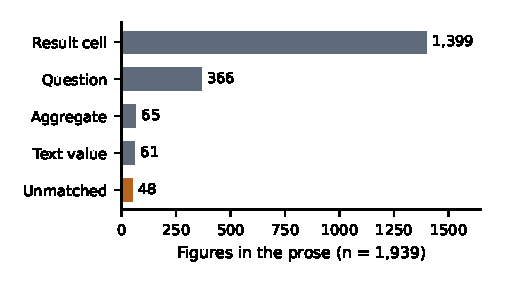
\includegraphics[width=0.92\columnwidth]{sources.pdf}
\caption{Sources of the figures in the pilot after the fixes. Traced figures matched a result cell (1,399), the question (366), a column aggregate (65) or a text value (61); 48 were unmatched.}\label{fig:sources}
\end{figure}

\paragraph{A flagged follow-up.} One flagged answer reads ``96,478 out of 99,441 \ldots{} 97.0\%''. Only 96,478 appears in the result of that turn. The other two figures were carried over from an earlier turn. Because 99,441 cannot be traced, the percentage cannot be derived from two traced figures either, and the answer is flagged. The reader is told that part of the sentence does not come from the data just retrieved, which is the intended behaviour. The figures may still be right. The checker reports that this turn did not establish them.

\paragraph{Caveat: in-sample.} The two defects were found and fixed on the same data on which the second run was measured. The 97.5\% and the 8 flags are therefore optimistic for unseen data. Numbered-list markers (``1.'', ``2.'') were also read as figures in a live answer and were fixed before this pilot. An out-of-sample evaluation is future work (Section~\ref{sec:plan}). The pilot also does not measure recall: it shows that few answers are flagged and that the flags it reviewed were justified, not that unflagged answers are correct.

\section{Planned Evaluation}\label{sec:plan}
The protocol was written on 30 September 2026, before any result on it was measured. Changes after data collection begins will be logged with the reason.

\paragraph{Research questions.}
\begin{description}
\item[RQ1] As a signal for ``this answer may be wrong'', how do data-level checks compare with model-based confidence in accuracy of the warning and in cost? Model-based baselines are self-consistency over $k=5$ samples, one LLM judge, and a two-provider judge ensemble.
\item[RQ2] Which check catches which error type, and which errors does none catch?
\item[RQ3] How often do the checks raise false alarms on correct answers?
\end{description}

\paragraph{Data.} (1) BIRD Mini-Dev, PostgreSQL version (500 questions, 11 databases; CC BY-SA 4.0), scored against the corrected annotations of Jin et al. \cite{jin2026}, who found annotation errors in 52.8\% of BIRD Mini-Dev. The original gold is used only as a sensitivity check. (2) A hand-built fan-out set of 60--100 questions on the same databases, whose natural SQL joins a one-to-many table under an aggregate, with gold SQL written and executed by hand; it is needed because BIRD rarely exercises fan-out. (3) The 30-question set above, as a case study only.

\paragraph{Conditions and baselines.} The system runs at shipped settings with the checks on. Signals compared are the tier, each check alone and combined; model-free baselines (executes without error, empty result, row count out of range); and the model-based baselines above, plus combinations of checks with a judge.

\paragraph{Metrics.} Correctness is execution match with the corrected gold, followed by manual review of every disagreement between that label and the checks, recording the error type (join or fan-out, filter value, column meaning, aggregation, time window, prose only). We report precision, recall and F1 of the warning for wrong answers; AUROC where a score exists; risk--coverage curves and selective accuracy at 80\% and 90\% coverage; false alarms on correct answers; and extra model calls and tokens (zero for the checks). Confidence intervals come from bootstrap resampling by question.

\paragraph{Hypotheses.}
\begin{description}
\item[H1] On join and aggregation errors, the checks have higher precision than an LLM judge at equal or lower cost. On other error types (wrong filter value, wrong column meaning) they catch little and the judge does better.
\item[H2] Checks combined with one judge beat either alone on risk--coverage.
\item[H3] Figure grounding flags fewer than 5\% of correct answers, and its catches are mostly prose errors rather than SQL errors.
\end{description}
Any outcome is reportable. A finding that the checks catch few real errors on BIRD would be a result.

\section{Related Work}
\paragraph{Predicting correctness.} Richardson \cite{richardson2026} is the closest work: it compares model-based signals and reports the AUROC values given in the introduction. We compare against the same families of signal but use signals computed from the executed result rather than from the model.

\paragraph{Benchmarks and their errors.} BIRD Mini-Dev \cite{birdminidev} has 500 questions over 11 databases, in SQLite, MySQL and PostgreSQL versions. Jin et al. \cite{jin2026} report annotation errors in 52.8\% of BIRD Mini-Dev and 62.8\% of Spider 2.0-Snow, and release corrected sets. This motivates our use of corrected annotations. Spider 2.0 \cite{lei2025} targets enterprise workflows, where an o1-preview based agent solves 21.3\%.

\paragraph{Templates.} TeCoD \cite{jivani2026} mines templates from labelled workloads, matches questions with natural language inference and decodes under a grammar. It reports up to 36\% higher execution accuracy than in-context learning and 2.2 times lower latency on matched queries. Our compiled tier is related in spirit but differs in source: templates derive from SQL the owner approved, and values are filled in code. We have not compared the two.

\paragraph{Semantic layers.} A dbt Labs blog post \cite{dbt2026blog} reports 98--100\% accuracy for a semantic layer in scope and 84--90\% for text-to-SQL on an 11-question set. It is vendor evidence on a very small set, and we cite it only as motivation.

\section{Limitations and Threats to Validity}\label{sec:limits}
\paragraph{Not yet measured.} No result here comes from an external benchmark. We have not measured the precision or recall of any check on known-wrong answers, nor compared any check with model-based confidence. The fan-out probe has not been evaluated, and the metric-reconciliation check named in the protocol is not built.
\paragraph{In-sample pilot.} The grounding checker was corrected on the data it was then measured on. The pilot also cannot detect wrong answers whose figures are all present in a wrong result, because grounding checks the prose against the result, not the query against the question.
\paragraph{Small baseline.} The baseline has 30 questions, one run, one SQL model (Groq gpt-oss-120b), and includes a synthetic corpus. Categories hold 6 to 10 questions each, too few for statistical claims. One miss is a defensible reading of an ambiguous question (which fulfillments form the denominator), scored wrong against a single reference.
\paragraph{Design bias.} The checks were designed with the StateSync data in view, so BIRD is the out-of-sample test. The fan-out set is built by the authors and will be reported separately and published. Execution-match labels have their own errors, which manual review of disagreements only partly limits. The vendor sources cited are not independent evidence.
\paragraph{Known coverage gap.} Fan-out under \texttt{COUNT(*)} is not covered yet, as one baseline miss shows.

\section{Conclusion}
We have described a text-to-SQL assistant whose trust signals are computed from the executed result: an evidence tier, three deterministic checks and figure grounding. On stored answers, figure grounding traced 97.5\% of figures and flagged 8 of 944 answers, all justified on manual review, but with defects tuned on the same data. The open question is whether such checks, evaluated out of sample on corrected BIRD Mini-Dev and a fan-out set, flag wrong answers more precisely and more cheaply than model-based confidence, and where they fail. The protocol and hypotheses are fixed in advance so that either outcome can be reported.

\begin{thebibliography}{9}\small
\bibitem{richardson2026} Richardson. What predicts correctness in text-to-SQL? A selective-prediction study. arXiv:2607.06799, 2026.
\bibitem{jin2026} Jin, Choi, Zhu, and Kang. Pervasive annotation errors break text-to-SQL benchmarks and leaderboards. arXiv:2601.08778, 2026.
\bibitem{lei2025} Lei et al. Spider 2.0. ICLR 2025. arXiv:2411.07763.
\bibitem{birdminidev} BIRD Mini-Dev (500 questions, 11 databases). \url{https://github.com/bird-bench/mini_dev}.
\bibitem{jivani2026} Jivani, Maheshwari, and Sarawagi. TeCoD. arXiv:2604.28028, 2026.
\bibitem{dbt2026blog} dbt Labs. Semantic layer vs text-to-SQL. Blog post, 2026.
\bibitem{dbt2026report} dbt Labs. 2026 report (survey of respondents on data-quality concerns), 2026.
\end{thebibliography}

\end{document}
